\section{Research Topics, Challenges, and New Ideas}

\begin{frame}
  \begin{center}
    {\color{Maroon}\Huge Research Directions and New Modeling Techniques}
  \end{center}
\end{frame}

%%%% ----------------------------
%%%%     CHALLENGES
%%%% ----------------------------

\begin{frame}
  \begin{center}
    {\color{Maroon}\Huge Challenges}
  \end{center}
\end{frame}

\begin{frame}{Are we there yet?}
  \begin{center}
    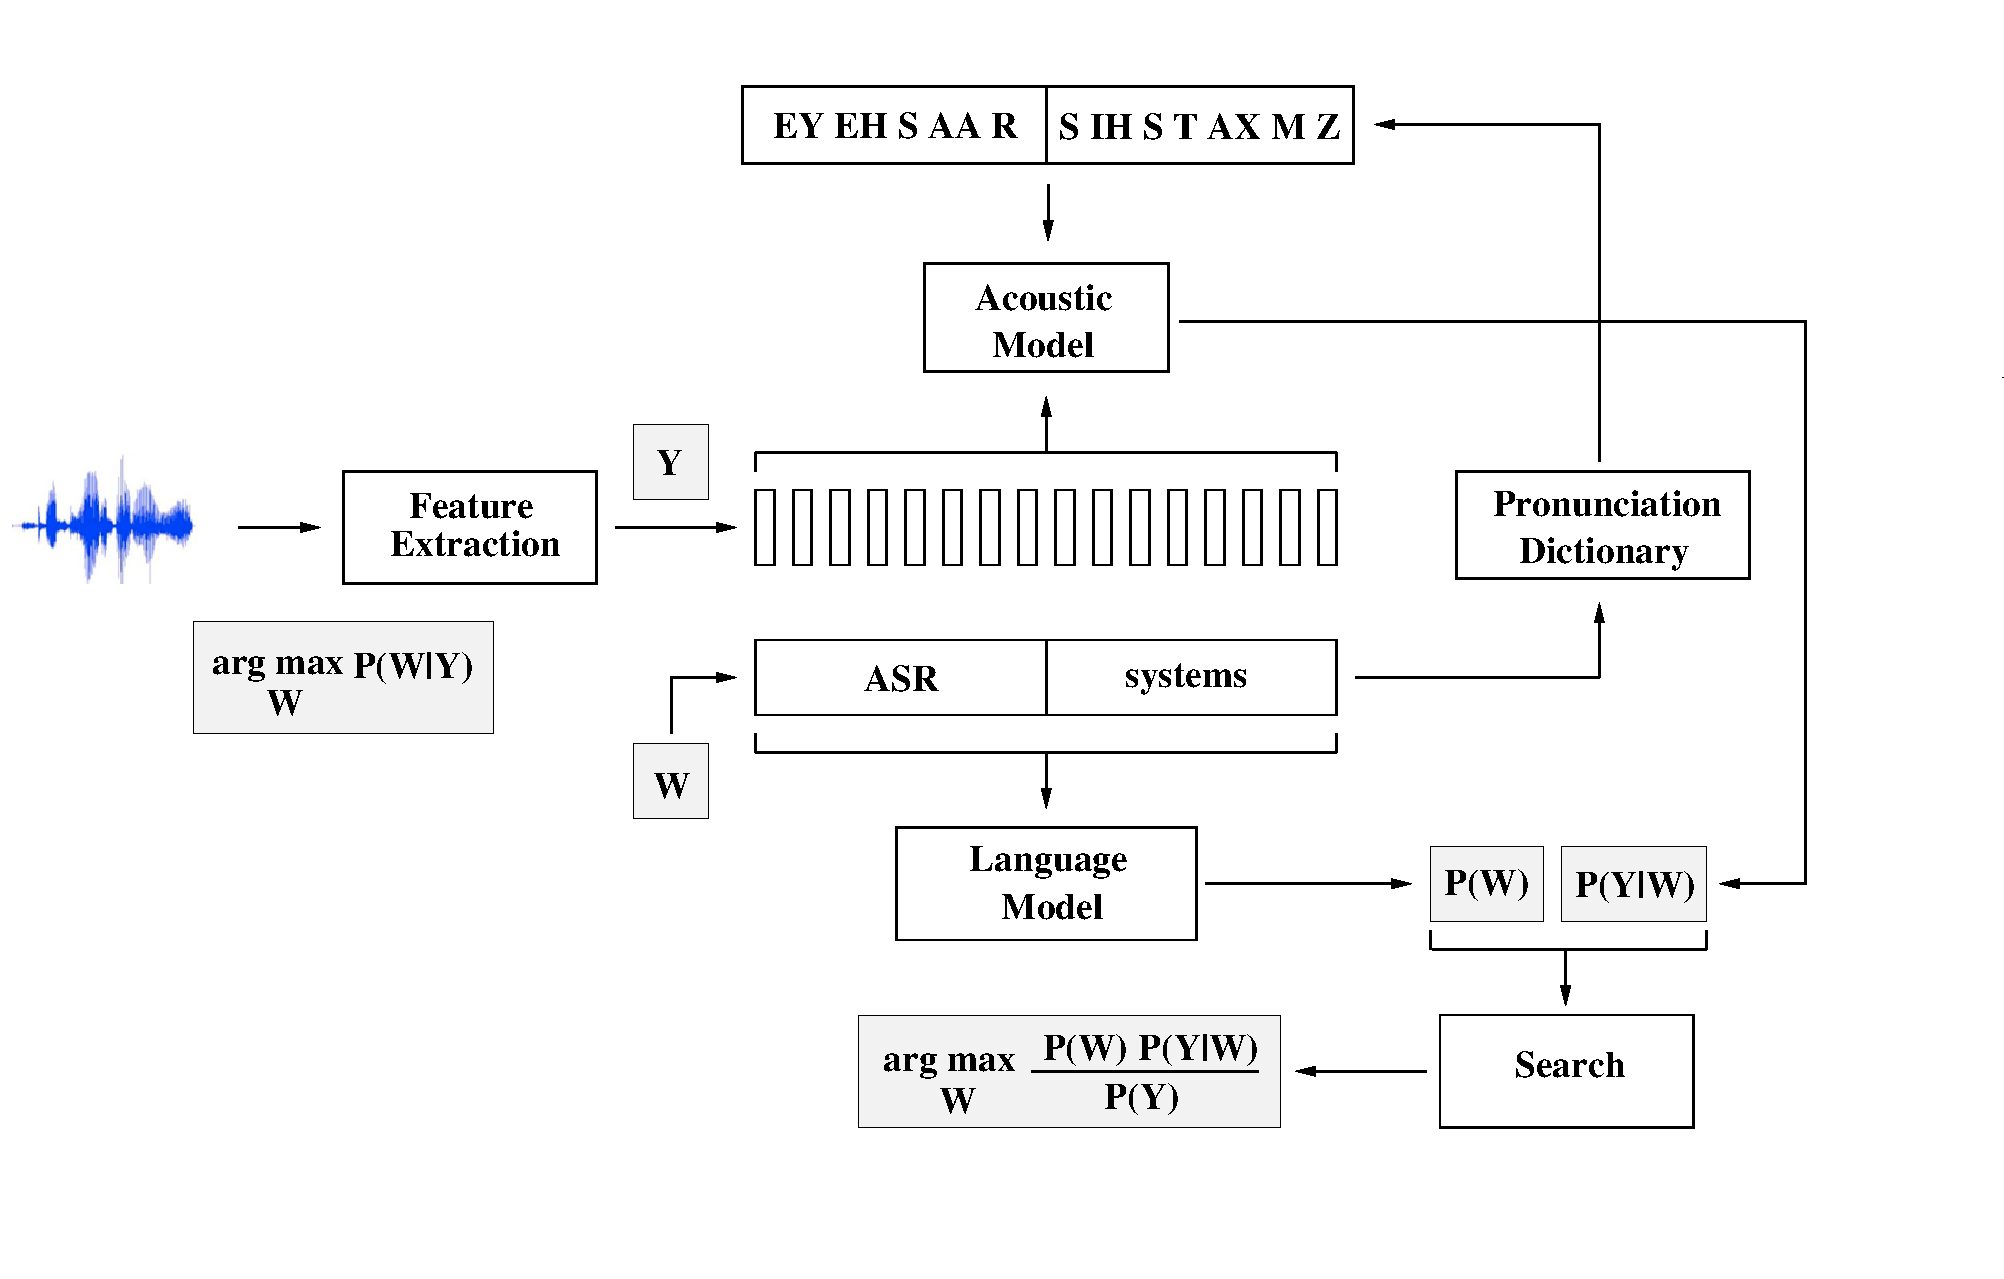
\includegraphics[height=77mm]{figures/ASR9}
  \end{center}
\end{frame}

\begin{frame}{Is that it?}
  \begin{center}
    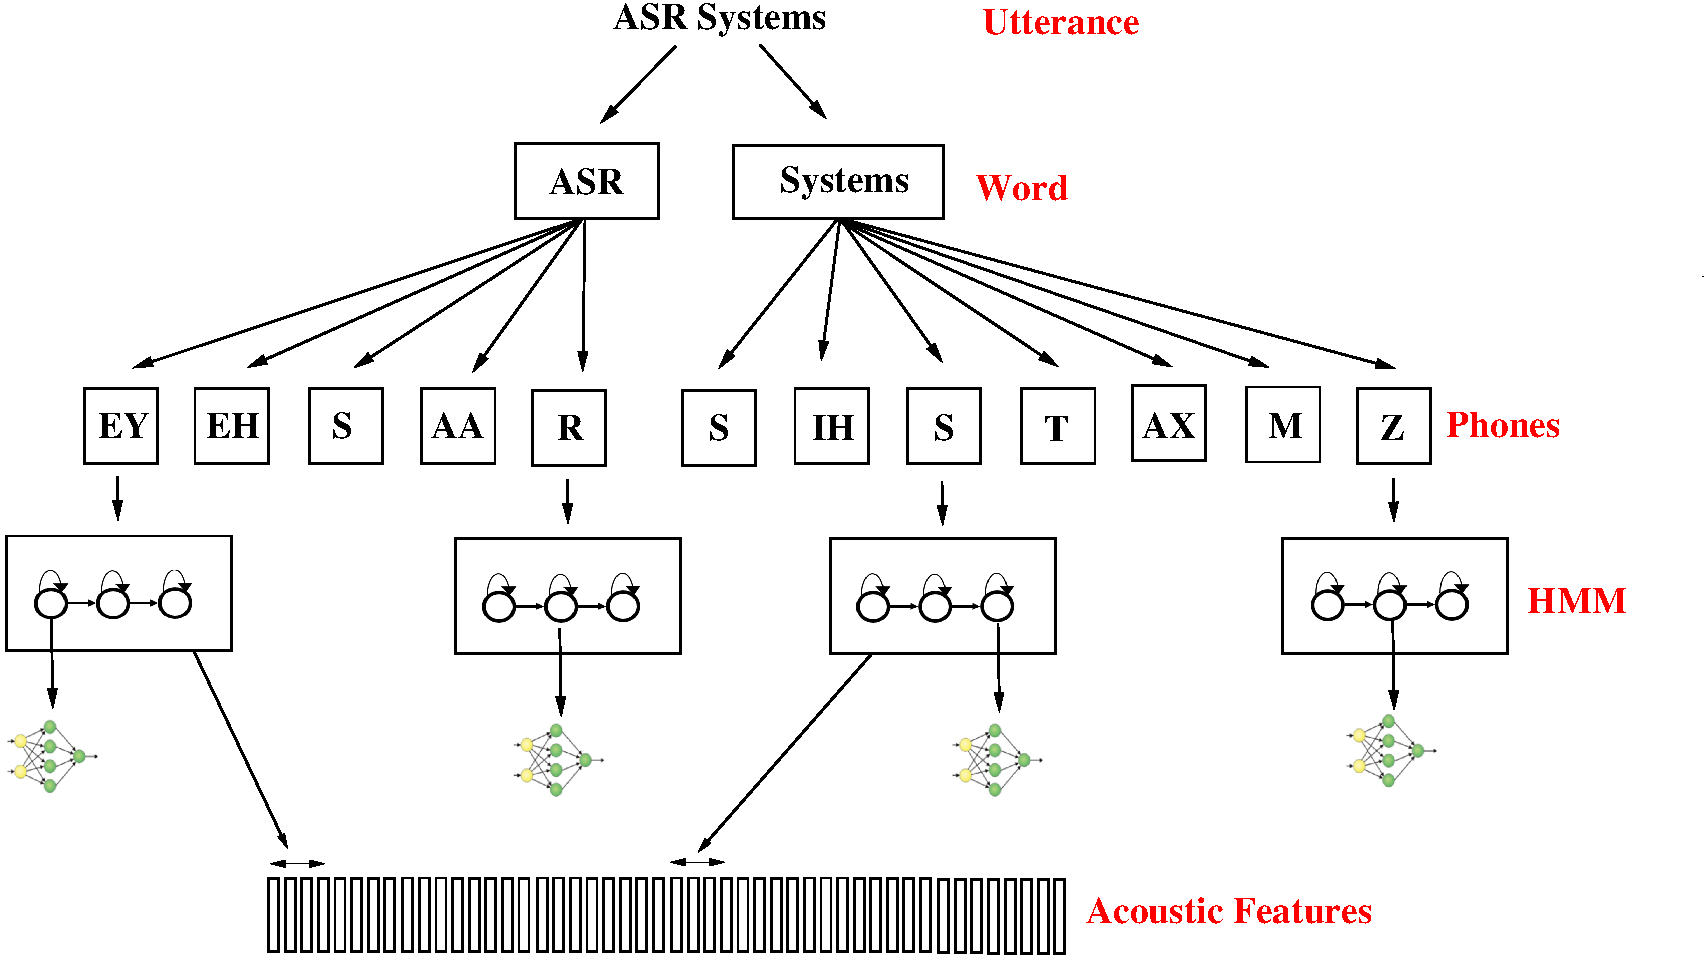
\includegraphics[height=65mm]{figures/am-mlp}
  \end{center}
\end{frame}

\begin{frame}{Challenges}
  \begin{itemize}
  \item What could be wrong?
  \item We are using a solid statistical framework, right?
  \item We know how to extract ``features''
  \item We know how to learn models
  \item We know how to search for the best path
  \end{itemize}
\end{frame}

\begin{frame}{Really?}
  \begin{itemize}
  \item Fundamental Equation of ASR
  \item $W' = argmax$
  \end{itemize}
\end{frame}

\begin{frame}
  \frametitle{Research Topics}
\end{frame}

\begin{frame}
  \frametitle{New Ideas}
\end{frame}

\section{End-to-End Systems}

\begin{frame}
  \frametitle{End-to-End Systems}
\end{frame}

\begin{frame}
  \begin{center}
    {\color{Maroon}\Huge Hands-On Experience with Virtual Machines}
  \end{center}
\end{frame}

\begin{frame}
  \frametitle{Practicalities}
  \begin{itemize}
  \item We want to give you hands-on experience with building ASR systems
  \item You will be able to train a system on a Babel language (most likely 201 Haitian)
  \item You can then experiment with other Babel languages, or port the system to other domains
  \item To facilitate experimentation, we will distribute a Virtual Machine (VM)
  \item \color{Maroon}Read on to see how you can prepare
  \end{itemize}
\end{frame}

\begin{frame}
  \frametitle{Virtual Machines and Tools}
  \begin{itemize}
  \item Think of a VM as a ``virtual'' computer, in our case running Linux
  \item VMs allow sharing reproducible experiments easily
  \item \url{https://github.com/srvk}, \url{http://speechkitchen.org} as repositories
  \item \url{https://www.vagrantup.com/} to build VMs
  \item \url{https://www.virtualbox.org/} to run VMs (along with \url{https://aws.amazon.com/})
  \item An ``image'' is a computer when it is turned off, it becomes an ``instance'' when you turn it on
  \end{itemize}
\end{frame}

\begin{frame}
  \frametitle{Exercises}
  \begin{itemize}
  \item We will share a Vagrantfile, plus an image on AWS (most likely), and/ or a Virtualbox OVA (less likely)
  \item Your best bet is to run the exercise on AWS
  \item So, you may want to sign up for an account first (\url{https://aws.amazon.com/getting-started/})
  \item Familiarize yourself with how to start a Linux VM on ``EC2'' using a pre-configured Amazon Machine Image (AMI)
  \item Training a DNN-based recognizer on a GPU will cost some money, but the cost should not be dramatic
  \item Once you reproduced the basics, you can continue on AWS, or you can migrate to your own infrastructure
  \end{itemize}
\end{frame}

\begin{frame}
  \frametitle{Eesen}
  \begin{itemize}
  \item We will use the ``Eesen'' toolkit (\url{https://github.com/srvk/eesen}) for end-to-end speech recognition
  \item It is based on Kaldi (\url{http://kaldi-asr.org/}), but a bit smaller and easier to handle
  \item \color{Maroon} More details to follow
  \end{itemize}
\end{frame}

\begin{frame}
  \frametitle{References}    
  \cite{quesst:icassp2015,metze:is2015,yajie-lstm:is2015,yajie-robust:is2015,yashesh:is2015,yajie:taslp2015,eesen,trecvid:2015,eesen-icassp,wang2016icassp,w4a:2016,icmr2016,miao:is2016,vms:is2016,shared:is2016,yash:is2016,e2echapter,dnnbook}
\end{frame}
